\chapter*{Appendix}
\addcontentsline{toc}{chapter}{Appendices}

\begin{figure}[h]
\caption{Font size range}
  \label{fig:fontSize}
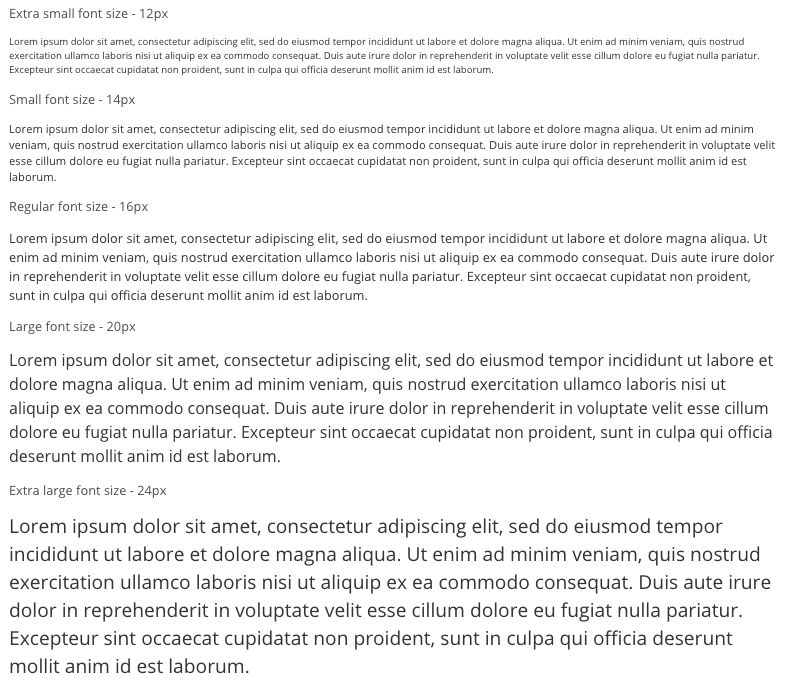
\includegraphics[scale=0.4]{../public/images/fontsizes}
\centering
\end{figure}

\begin{figure}[h]
\caption{Text Alignments}
  \label{fig:textalign}
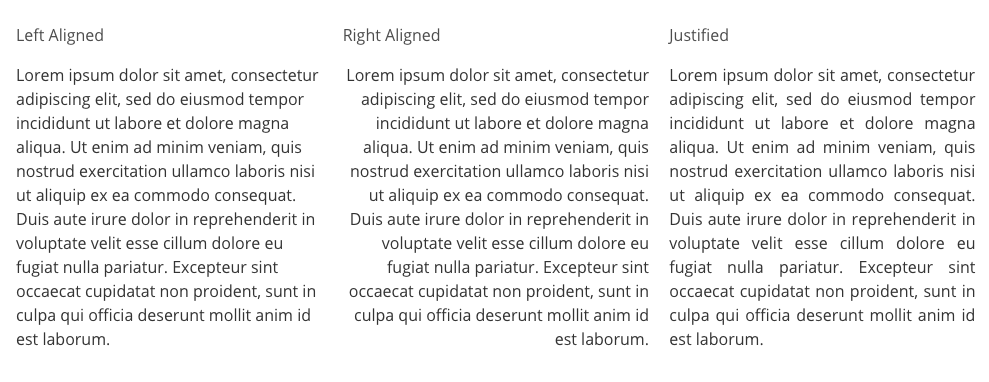
\includegraphics[scale=0.3]{../public/images/text-align}
\centering
\end{figure}

\begin{figure}[h]
\caption{Font Weighting}
  \label{fig:fontweight}
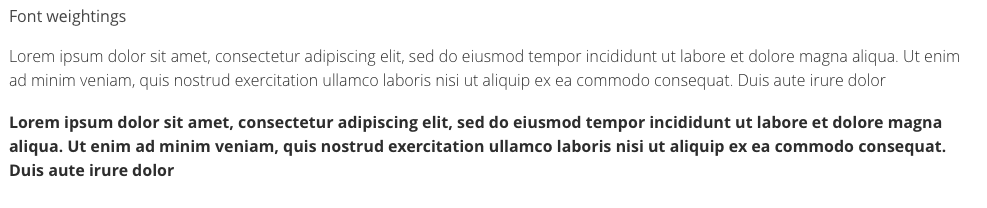
\includegraphics[scale=0.4]{../public/images/font-weighting}
\centering
\end{figure}

\begin{figure}[h]
\caption{Generic Button Types}
  \label{fig:genButtons}

\includegraphics[scale=0.5]{../public/images/generic-buttonsa}
\centering
\end{figure}



\begin{figure}[h]
\caption{Button Modifiers}
  \label{fig:buttonMods}

\includegraphics[scale=0.5]{../public/images/button-modifiers}
\centering
\end{figure}

\begin{figure}[h]
\caption{Alerts}
  \label{fig:alerts}
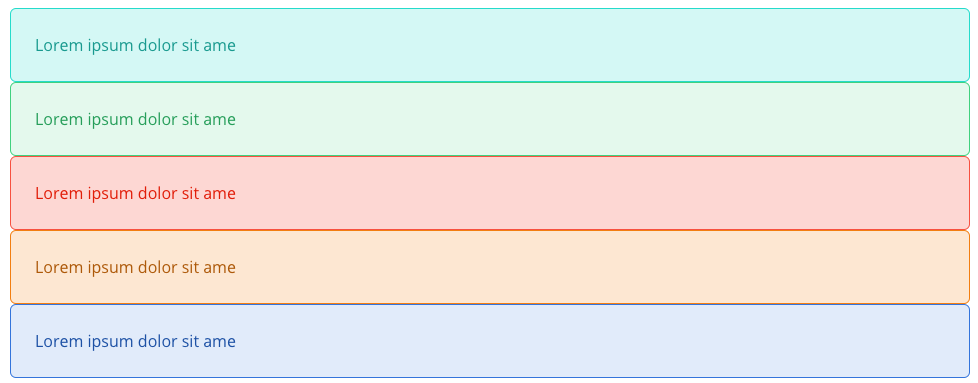
\includegraphics[scale=0.3]{../public/images/alertd}
\centering
\end{figure}

\begin{figure}[h]
\caption{Alert Modifiers}
  \label{fig:AlertModifiers}
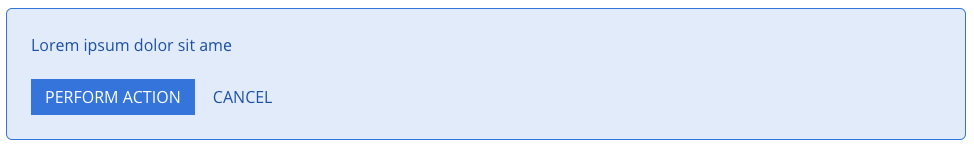
\includegraphics[scale=0.3]{../public/images/addtoalert}
\centering
\end{figure}

\begin{figure}[h]
\caption{Tables with Modifiers}
  \label{fig:tableMod}
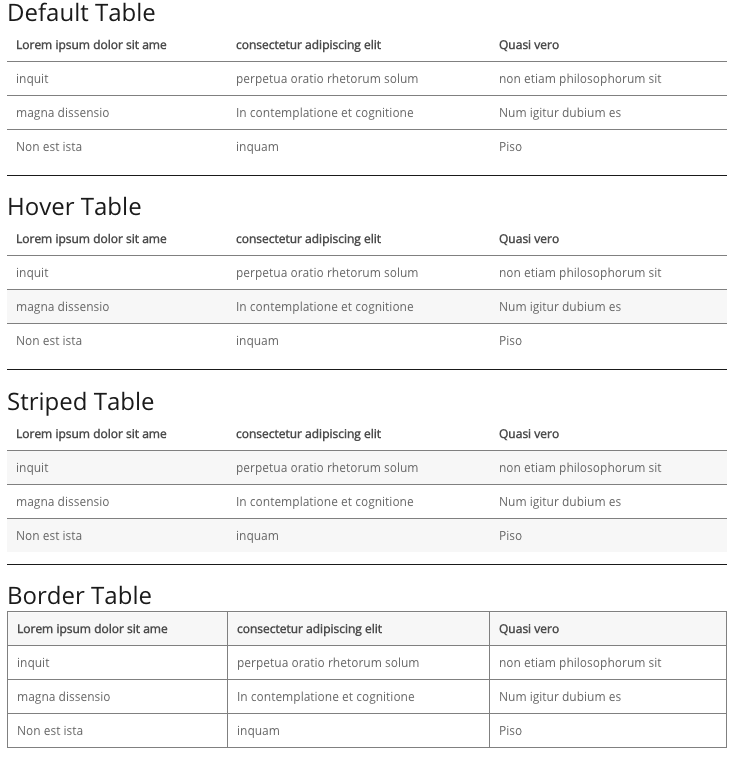
\includegraphics[scale=0.4]{../public/images/tables}
\centering
\end{figure}

\begin{figure}[h]
\caption{Table With Other Class Modifiers}
  \label{fig:tableClass}
  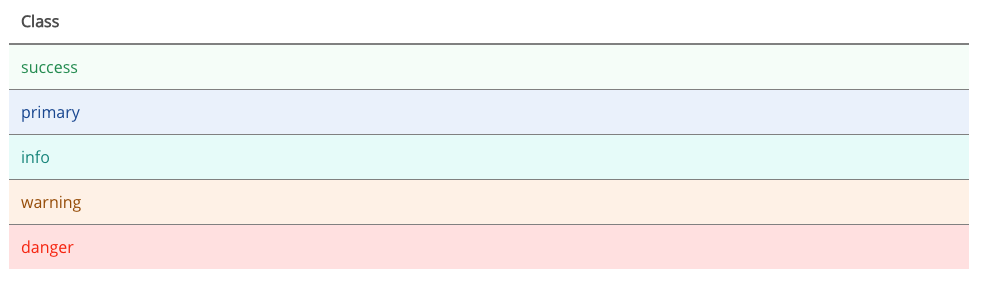
\includegraphics[scale=0.3]{../public/images/tableClass}
\centering
\end{figure}

\begin{figure}[h]
\caption{Default Panel}
  \label{fig:panel}
  
\includegraphics[scale=0.4]{../public/images/panel}
\centering
\end{figure}

\begin{figure}[h]
\caption{Panel with modifiers}
  \label{fig:panelmod}
  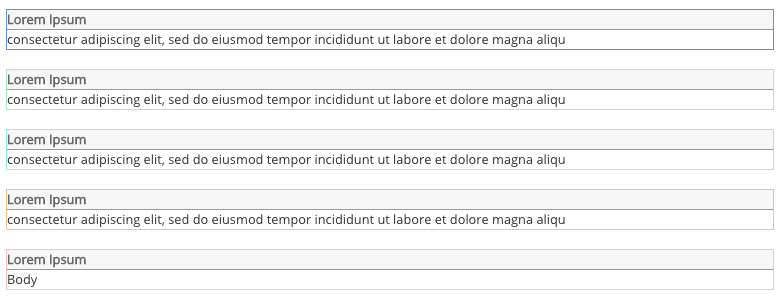
\includegraphics[scale=0.4]{../public/images/panelmod}
\centering
\end{figure}

\begin{figure}[h]
\caption{Labels}
  \label{fig:label}
  
\includegraphics[scale=0.5]{../public/images/labels}
\centering
\end{figure}

\begin{figure}[h]
\caption{Jumbotron}
  \label{fig:jumbo}
  
\includegraphics[scale=0.4]{../public/images/jumbrotron}
\centering
\end{figure}

\begin{figure}[h]
\caption{Default Button Group}
  \label{fig:defualtgroup}

\includegraphics[scale=0.5]{../public/images/button-group=defualt}
\centering
\end{figure}

\begin{figure}[h]
\caption{Button Group Sizes}
  \label{fig:groupSize}
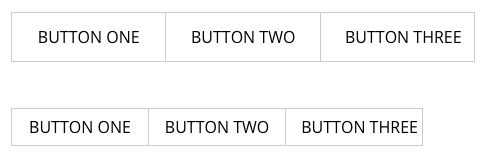
\includegraphics[scale=0.5]{../public/images/button-group-size}
\centering
\end{figure}


\begin{figure}[h]
\caption{Button Group With Modifiers}
  \label{fig:modButtonGroup}

\includegraphics[scale=0.5]{../public/images/buttongroups}
\centering
\end{figure}

\begin{figure}[h]
\caption{Form elements}
  \label{fig:form}
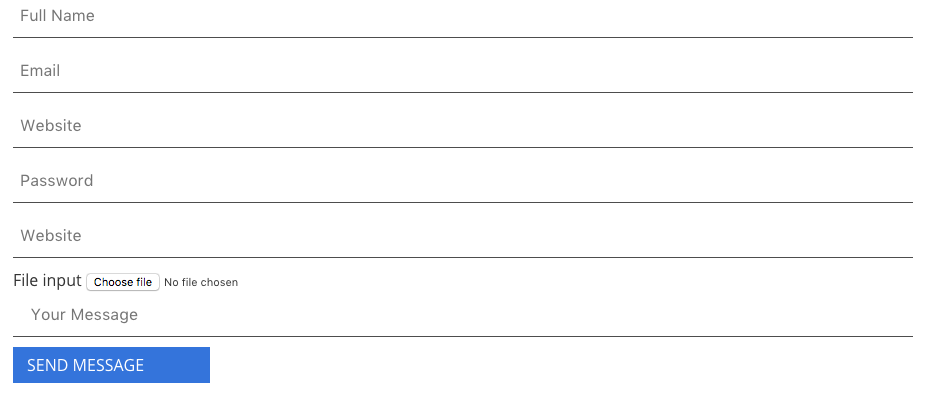
\includegraphics[scale=0.3]{../public/images/form}
\centering
\end{figure}


\begin{figure}[h]
\caption{Radio Buttons and Checkboxes}
  \label{fig:radio}

\includegraphics[scale=0.5]{../public/images/radio}
\centering
\end{figure}


\begin{figure}[h]
\caption{12 Column Layout}
  \label{fig:columnlayout}
  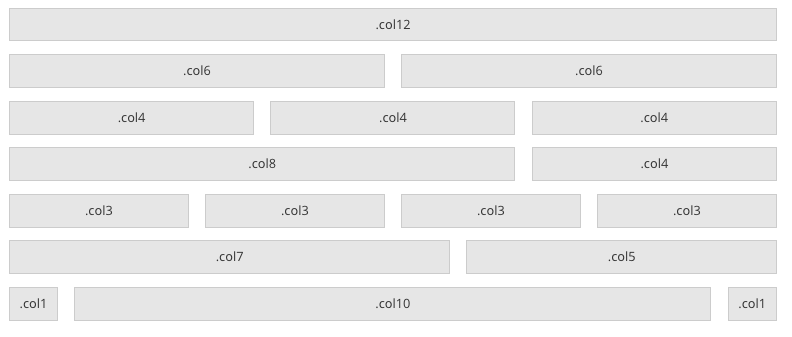
\includegraphics[scale=0.4]{../public/images/columnlayout}
\centering
\end{figure}

\begin{figure}[h]
\caption{Blockquote}
  \label{fig:quote}
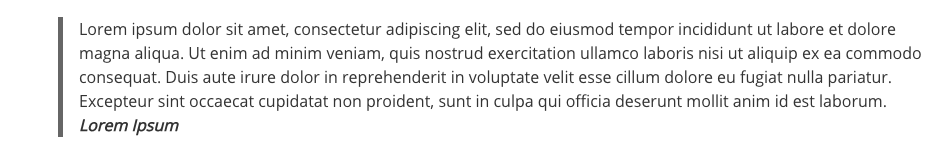
\includegraphics[scale=0.4]{../public/images/blockquote}
\centering
\end{figure}


\begin{figure}[ht]
\caption{Nunjucks File Structure}
  \label{fig:structure}
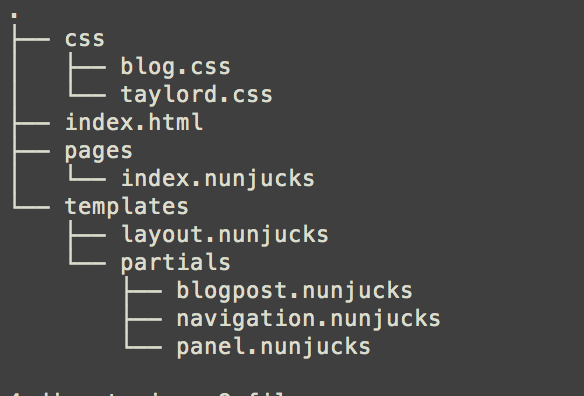
\includegraphics[scale=0.5]{../public/images/fileStructure}
\centering
\end{figure}

\begin{figure}[ht]
\caption{12 grid layout with the 960 grid}
  \label{fig:grid}
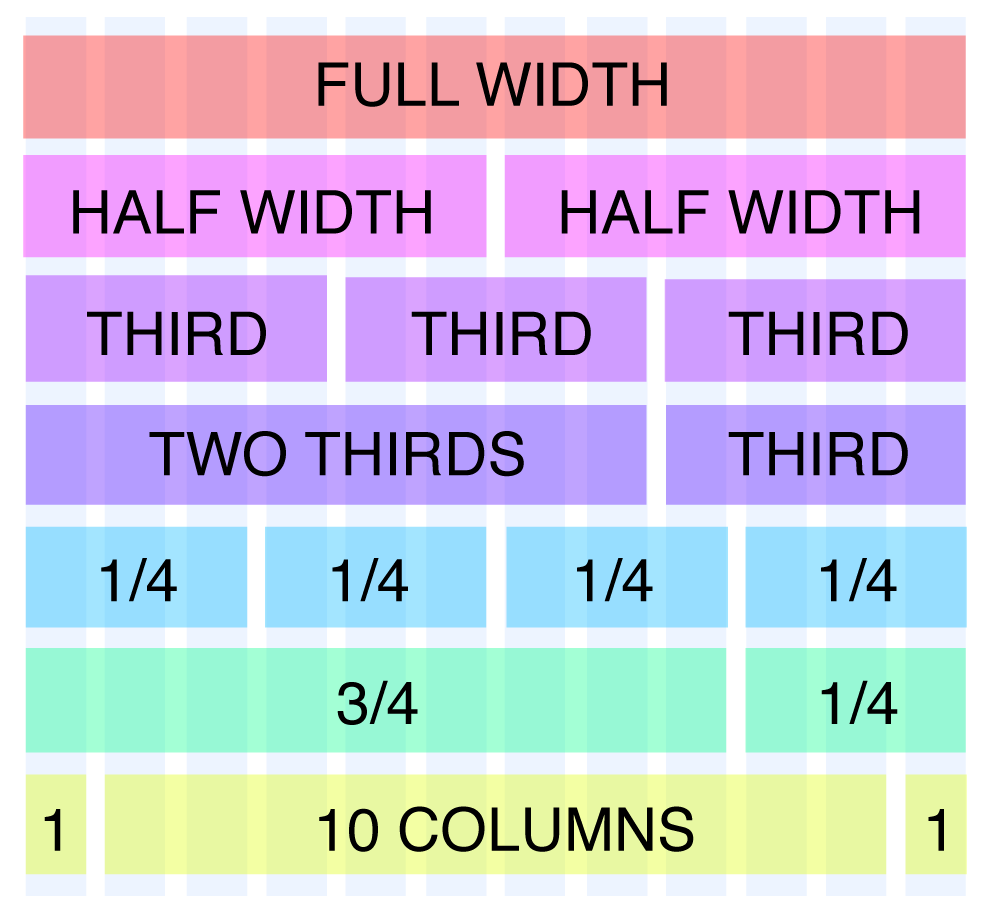
\includegraphics[scale=0.2]{../public/images/960-12-col-grid}
\centering
\end{figure}

\begin{figure}[ht]
\caption{Chrome Developer Tools}
  \label{fig:tools}
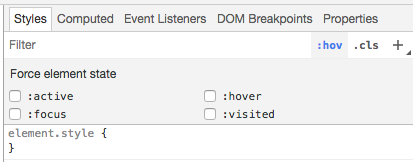
\includegraphics[scale=0.5]{../public/images/tools}
\centering
\end{figure}


\newpage
\begin{table}[!ht]
\centering
\caption{Framework features}
\label{features}
\begin{tabular}{llll}
 & Bootstrap & Foundation & Skeleton \\
Alerts & Yes & Yes & No \\
Accordion & Yes & Yes & No \\
Badges & No & Yes & No \\
Breadcrumbs & Yes & Yes & No \\
Buttons & Yes & Yes & Yes \\
Carousel & Yes & Yes & No \\
Dropdown & Yes & Yes & No \\
Forms & Yes & Yes & Yes \\
Form Validation & Yes & Yes & No \\
Grid & Yes & Yes & Yes \\
Icons & No & Yes & No \\
Labels & Yes & Yes & No \\
Lists & Yes & Yes & Yes \\
Media Object & Yes & Yes & Yes \\
Modals & Yes & Yes & No \\
Navigation & Yes & Yes & No \\
Pagination & Yes & Yes & No \\
Panels & Yes & Yes & No \\
Popovers & Yes & Yes & No \\
Print Styles & Yes & Yes & Yes \\
Progress Bar & Yes & Yes & No \\
Responsive Media & No & Yes & No \\
Right to Left & No & Yes & No \\
Scrollspy & Yes & Yes & No \\
Tables & Yes & Yes & Yes \\
Tabs & Yes & Yes & No \\
Thumbnails & Yes & Yes & No \\
Tooltips & Yes & Yes & No \\
Typeahead & No & No & No \\
Typography & Yes & Yes & Yes \\
Video Scaling & Yes & Yes & No
\end{tabular}
\end{table}

\begin{table}
\centering
\caption{Column Layout}
\label{column}
    \begin{tabular}{lll}
    Layout  & ~ & Number of Columns \\
    2 x 480 & ~ & 2 columns         \\
    3 x 320 & ~ & 3 columns         \\
    4 x 240 & ~ & 4 columns         \\
    5 x 192 & ~ & 5 columns         \\
    6 x 160 & ~ & 6 columns         \\
    8 x 120 & ~ & 8 columns         \\
    10 x 96 & ~ & 10 columns        \\
    12 x 80 & ~ & 12 columns        \\
    16 x 60 & ~ & 16 columns        \\
    20 x 48 & ~ & 20 columns        \\
    24 x 50 & ~ & 24 columns        \\
    30 x 32 & ~ & 30 columns        \\
    \end{tabular}
\end{table}